\chapter{Ausgangssituation}
\label{cha:Ausgangssituation}


\section{Monitoring über MQTT.fx}
    Die grafische und leicht verständliche, aber gleichzeitig leistungsfähige Anwendung MQTT.fx wird bisher für das Testen und Debuggen von MQTT-basierter Kommunikation verwendet.
    Sie wird verwendet, um die Nachrichtenflüsse zwischen Clients und Broker sichtbar zu machen \autocite{MQTTfxGrafischesWerkzeug}. Diese Software ist eine von zwei Möglichkeiten
    bei MULTIVAC, den MQTT-Nachrichtenverlauf darzustellen und auch Nachrichten zu simulieren. 
    \subsection{Funktionalität von MQTT.fx}
        MQTT.fx ist ein grafischer Desktop-Client für das MQTT-Protokoll. Die Anwendung verbindet sich als MQTT-Client mit dem externen Broker.
        Beim Verbinden erlaubt die Applikation das Anlegen wiederverwendbarer Verbindungsprofile. Konfigurierbare Parameter sind dabei die Broker-Adresse, Port, Client-ID, 
        MQTT-Version, Clean-Session, Keep-Alive-Zeit, Authentifizierung durch Benutzername und Passwort und eine TLS/SSL-Verschlüsselung. \autocite{ouyangMQTTfxGuideFeatures}

        Über einen Reiter Publish lassen sich Nachrichten über frei definierbare Topics versenden. Dazu lassen sich auch das QoS-Level und die Retain-Flag manuell einstellen. 
        Nachrichten können ähnlich wie Verbindungsprofile über Vorlagen oder die Historie wiederverwendet werden. So können Sensorwerte, Statusmeldungen und Steuerbefehle 
        simuliert werden \autocite{ConnectMQTTfxEMQX}.
        
        \begin{figure}[htbp]
            \centering
            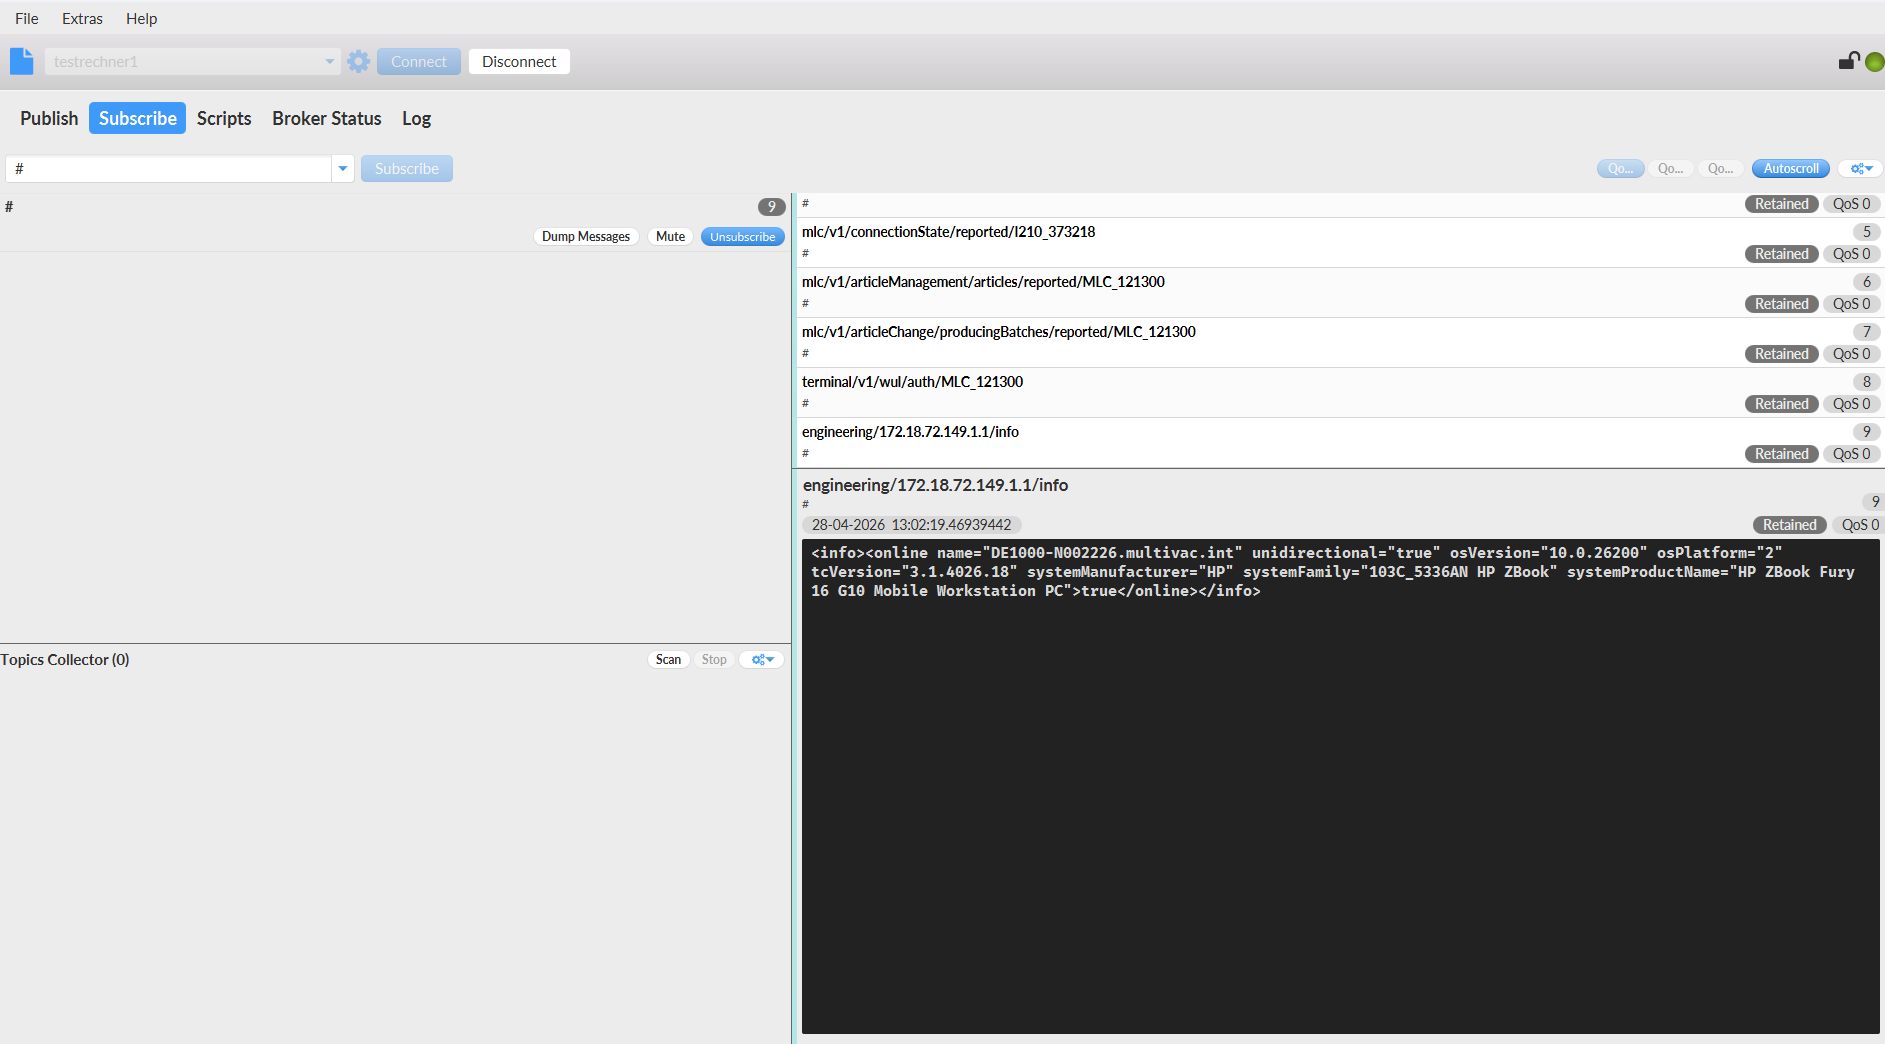
\includegraphics[width=0.8\textwidth]{images/mqttfx_subscribe.png}
            \caption{Subscribe-Reiter in MQTT.fx}
            \label{fig:mqttfx_subscribe}
        \end{figure}

        Neben dem Publish-Reiter verfügt \textit{MQTT.fx} auch über einen Subscribe-Reiter, der in Listing \ref{fig:mqttfx_subscribe} dargestellt ist. Hier können einzelne Topics oder Topic-Hierarchien abonniert werden.
        Die Darstellung der empfangenen Nachrichten unter den abonnierten Topics erfolgt dann in Echtzeit und mit den relevanten Metadaten Topic, Payload, \acrshort{acr:QoS} und Empfangszeitpunkt. \autocite{ouyangMQTTfxGuideFeatures}

        Darüber hinaus verfügt das Programm über eine Logging- und Analysefunktion. Dieser Reiter ist mit einem integrierten Log-Fenster ausgestattet, welches den Verbindungsaufbau und -abbau, Subscribe- und Publish-Events, MQTT-Nachrichten sowie Broker-Statusmeldungen protokolliert. \autocite{ouyangMQTTfxGuideFeatures}

        Eine weitere wichtige Funktion stellt die Skript- und Automatisierungsfunktion dar. MQTT.fx stellt eine einfache Java-basierte Skript-Schnittstelle bereit. 
        Diese ermöglicht automatisiertes Publizieren bestimmter Nachrichtenverläufe, die manuell durch einen Java-Programmcode erstellt werden können \autocite{MQTTTestingDebugging}.

        Zuletzt wird neben den zuvor genannten Reitern der Broker-Status angezeigt. In diesem werden grundsätzliche Informationen über die Anzahl der verbundenen Clients, Anzahl an gesendeten Nachrichten und weitere ähnliche Daten des Brokers angezeigt. \autocite{ouyangMQTTfxGuideFeatures}

        MQTT.fx stellt eine umfangreiche Sammlung von Funktionen zur Verfügung, die insbesondere für das Testen, Debuggen und Analysieren von MQTT-Kommunikation geeignet sind \autocite{MQTTTestingDebugging}. 
        Der Funktionsumfang ist dabei bewusst auf die Rolle eines Client-Werkzeugs ausgelegt, wobei der produktive Einsatz als dauerhaftes Monitoring- oder Visualisierungssystem nicht intendiert ist.
    \subsection{Gründe für und gegen den Einsatz von MQTT.fx}
        Diese Applikation ermöglicht es Entwicklern, ohne eigene Implementierung Publisher- und Subscriber-Rollen zu simulieren. 
         Ein klarer Vorteil bei MQTT.fx ist die mögliche Darstellung von Clean Session, 
        Last-Will-Nachrichten, QoS-Level oder Retained Messages. Darüber hinaus bietet MQTT.fx umfangreiche Logging- und Visualisierungsfunktionen, wodurch falsche Zustandsannahmen 
        oder Timing-Probleme schnell erkannt werden können.
        MQTT.fx bietet zudem unterschiedliche Payload-Decoder, wodurch eine bessere Analyse verschiedener MQTT-Nachrichten, ohne eigene Interpretation dieser, möglich 
        ist \autocite{MQTTTestingDebugging}.
         
        In der praktischen Exploration konnten jedoch auch folgende Nachteile erkannt werden. MQTT.fx speichert die empfangenen Nachrichten nicht dauerhaft. Eine langfristige Analyse ist dadurch nur durch manuelles Kopieren der Logs in externe Applikationen möglich.
        Außerdem ist MQTT.fx nur auf die Anzeige einzelner Subscriptions fokussiert. Deshalb ist die Darstellung zusammenhängender Nachrichtenflüsse über mehrere Topics hinweg 
        sehr eingeschränkt und erschwert die Analyse komplexer Topic-Hierarchien, wie sie in Automatisierungssystemen häufig auftreten.
        Ein weiterer zentraler Punkt, der gegen die Nutzung von MQTT.fx spricht, ist die Konzipierung als eigenständige Desktop-Anwendung. Deswegen ist eine Integration
        in bestehende \gls{acr:HMI} oder produktive Visualisierungssysteme nicht möglich. Außerdem gibt es keine Möglichkeit zur Weiterverarbeitung von Daten, 
        systematischen Auswertung von Tests oder zur Integration externer Datenquellen. Dadurch werden sowohl die Analyse als auch die Simulation bestimmter Szenarien eingeschränkt.

\section{Monitoring über \acrshort{acr:MQTT} Explorer}
    Eine weitere Möglichkeit für das Auslesen von MQTT-Nachrichten bietet \textit{MQTT Explorer} \autocite{MQTTExplorer}. Dieser bietet gegenüber MQTT.fx zusätzliche Funktionen und ist insgesamt übersichtlicher sowie stärker auf den Anwendungsfall ausgerichtet. Aus praktischen Explorationen konnten seine Funktionen sowie Vor- und Nachteile festgestellt werden.

    \begin{figure}[htbp]
        \centering
        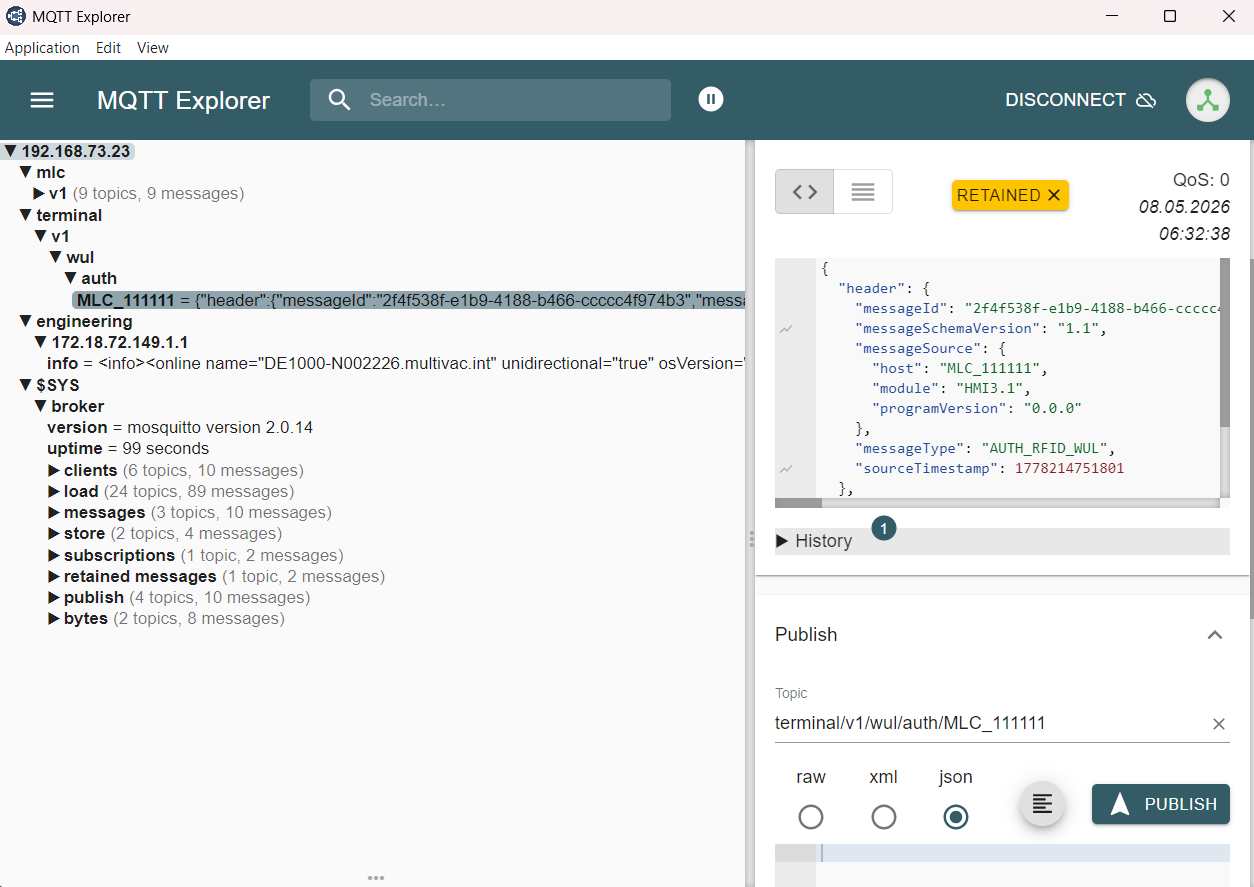
\includegraphics[width=0.7\linewidth]{images/MQTTexplorer.png}
        \caption{MQTT Explorer}
        \label{fig:MQTTexplorer}
    \end{figure}

    Wie in der Abbildung \ref{fig:MQTTexplorer} zu sehen ist, listet dieser alle erkannten Topics automatisch in einer Baumstruktur auf. Dies funktioniert durch das Aufspalten der Topics in die einzelnen Hierarchischen Topic-Ebenen. Dadurch ist ein ausgiebiges Wissen über die Topicstruktur oder ein vorheriges Scannen von Topics wie bei MQTT.fx nicht erforderlich, damit man die Nachrichten topic-bezogen filtern kann. Auf der rechten Seite befindet sich dann zum einen ein Nachrichtenfenster, in dem die angeklickte Nachricht in der Baumstruktur angezeigt wird. Zum anderen kann man dort auch Nachrichten selbst unter einem selbst eingegebenen Topic publizieren.

    Ein wesentlicher Vorteil gegenüber MQTT.fx ist die Möglichkeit der Volltextsuche, die in der Abbildung \ref{fig:MQTTexplorer} oben als Sucheingabe-Feld zu sehen ist. Durch das Eingeben eines Begriffs werden nur noch die Nachrichten in der Baumstruktur angezeigt, die den Suchbegriff enthalten. So wird die Suche erheblich vereinfacht.  

    Ein großer Nachteil ist jedoch die eingeschränkte Übersichtlichkeit des Nachrichtenverlaufs. Er lässt sich zwar durch die sogenannte Historie anzeigen. Diese beschränkt sich dann aber nur auf ein gezieltes Topic, wodurch die Reihenfolge aller Nachrichten nicht vollständig nachvollzogen werden kann. Auch die Volltextsuche beschränkt sich nur auf aktuelle Nachrichten und kann vergangene Nachrichten nicht weiter nachvollziehen. 

    Dadurch wird die Analyse von Datenströmen, bei denen die Reihenfolge eingehender Nachrichten eine entscheidende Rolle spielt, deutlich erschwert. Aufgrund dessen erfüllt auch diese Applikation die definierten Anforderungen nicht.
\section{Möglichkeit der Nutzung und Erweiterung bereits existenter Applikationen}
    Eine weitere Möglichkeit neben der Verwendung von bereits fertigen Programmen ist die Weiterentwicklung existenter Applikationen, die den Programmcode veröffentlichen. Eine hierfür besonders geeignete Applikation ist \textit{MQTTMultimeter}. Da der Quellcode von \textit{MQTTMultimeter} öffentlich verfügbar ist, konnten zentrale Komponenten der Anwendung praktisch analysiert und hinsichtlich ihrer Erweiterbarkeit bewertet werden. Die Analyse basiert auf dem auf GitHub veröffentlichten Projektstand \autocite{zotero-item-198}.
\subsection{Funktionsweise von MQTTMultimeter}
    \textit{MQTTMultimeter} erweist sich als eine schon sehr ausgereifte Applikation zum Anzeigen von MQTT-Nachrichten. Dieses Programm bietet eine geeignete Kombination aus MQTT.fx und dem \acrshort{acr:MQTT} Explorer. Es hat einen Reiter für die Anzeige der Baumstruktur, die sehr ähnlich funktioniert wie bei dem \acrshort{acr:MQTT} Explorer (siehe Abbildung \ref{fig:Baumstruktur}). Auch hier lässt sich der Nachrichtenverlauf nur durch eine Historie eines einzelnen Topics darstellen. 
    \begin{figure}[htbp]
        \centering
        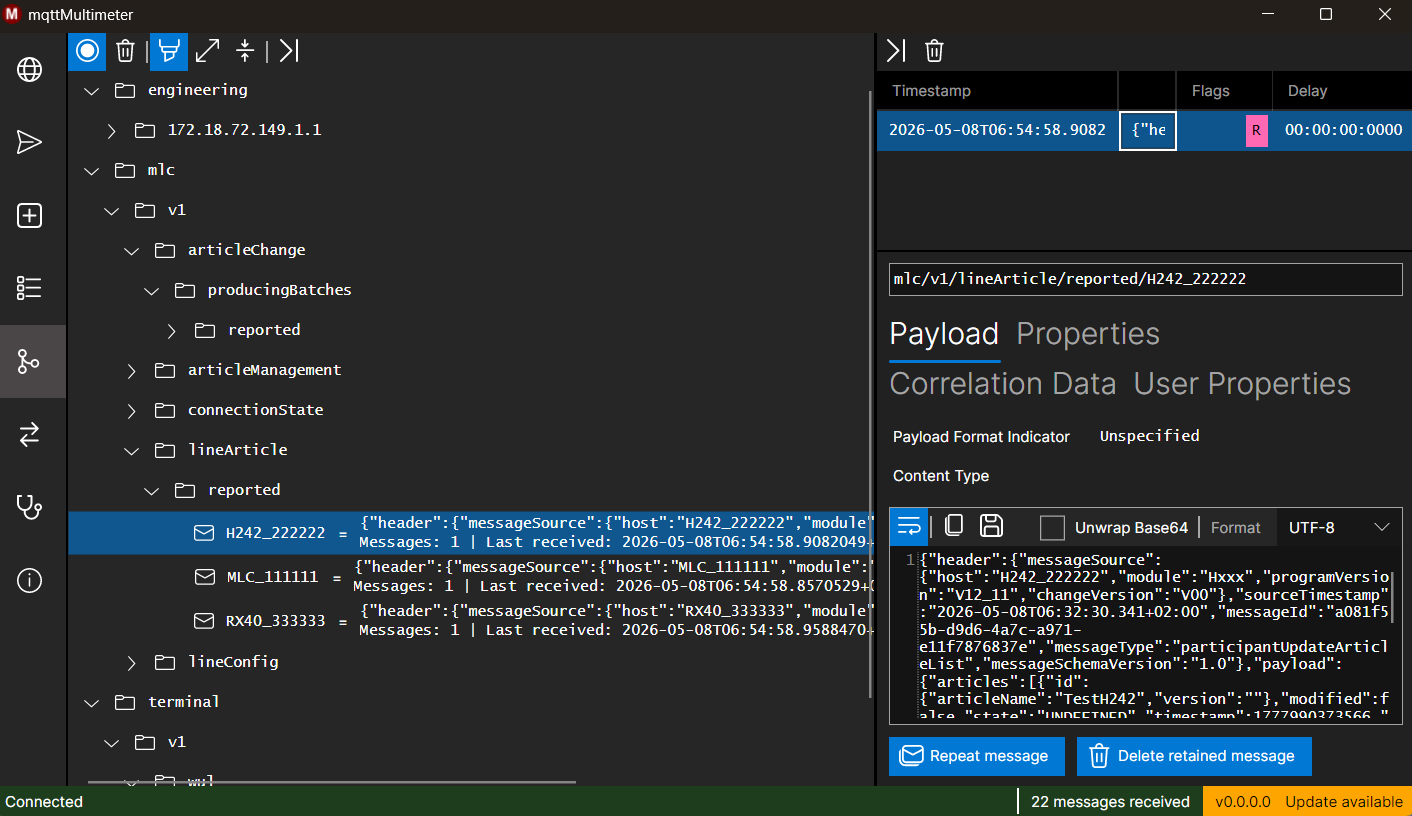
\includegraphics[width=0.9\linewidth]{images/MQTTMultimeter.png}
        \caption{Anzeigen der Nachrichten in einer Baumstruktur im MQTTMultimeter}
        \label{fig:Baumstruktur}
    \end{figure}

    In einem anderen Reiter können dann die Nachrichten in ihrer zeitlichen Empfangsreihenfolge angezeigt werden. Der Vorteil hier gegenüber MQTT.fx ist das Filtern nach Topics durch eine Eingabe oben (siehe Abbildung: \ref{fig:Nachrichtenverlauf}). Durch einen Klick auf das ausgewählte Topic wird die Nachricht sowie auch weitere Informationen zur Nachricht rechts angezeigt. Hier können die Nachrichten auch in einen Ordner abgelegt werden, jedoch auch nur wieder von der Applikation selbst aufgerufen werden.  

    In der Baumstruktur wie auch in beim Nachrichtenverlauf kann die angezeigte Nachricht direkt in den Publish Reiter kopiert werden. Dort kann die Nachricht selbst versendet werden, wodurch das Simulieren von Nachrichten vereinfacht wird.

    \begin{figure}[htpb]
        \centering
        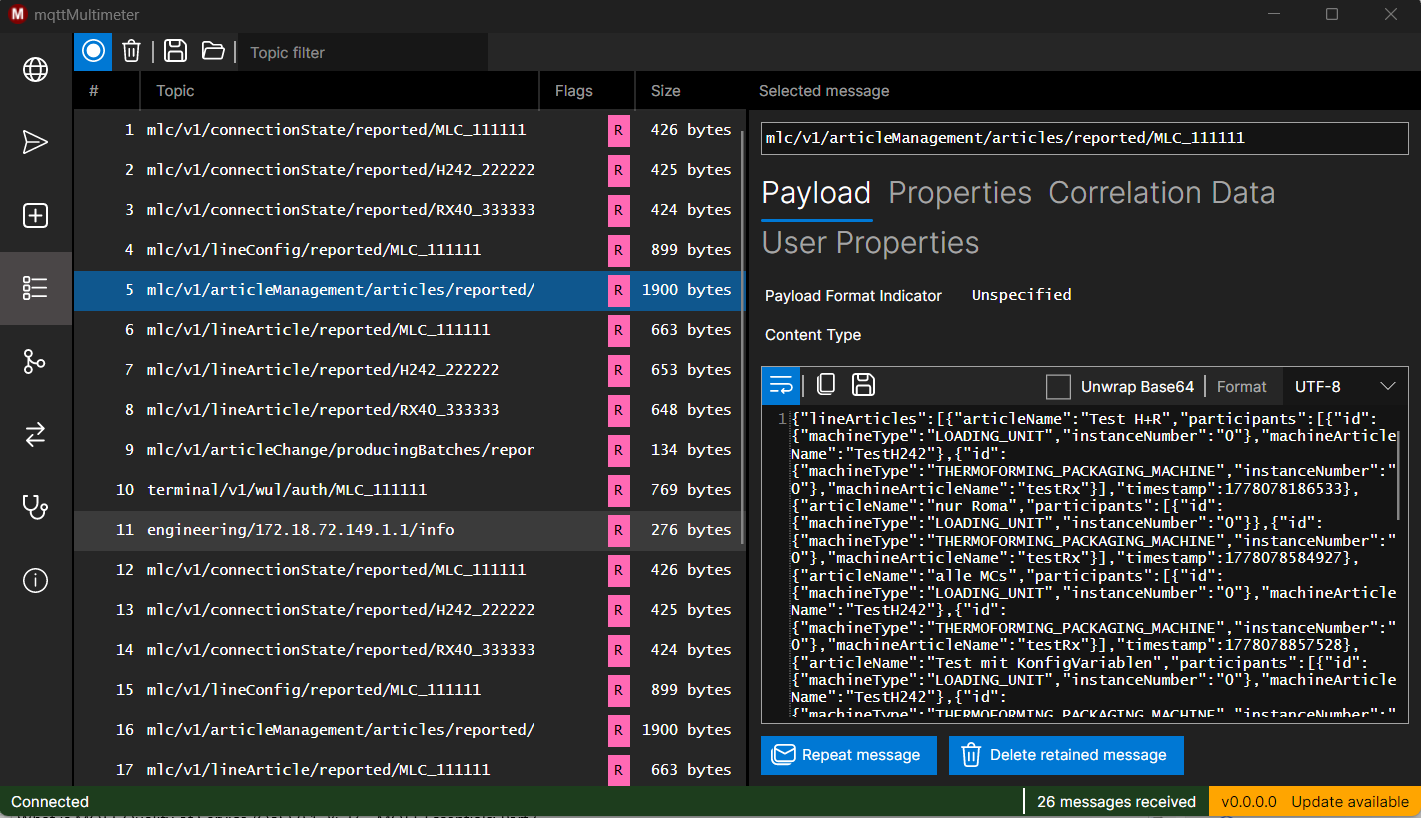
\includegraphics[width=0.9\linewidth]{images/MQTTMultimeterInflight.png}
        \caption{Nachrichtenverlauf im MQTTMultimeter}
        \label{fig:Nachrichtenverlauf}
    \end{figure}

    Ein Nachteil dieser Applikation ist die teilweise komplexe Benutzeroberfläche. Während beim MQTT Explorer die Nachrichten automatisch nach dem Verbinden angezeigt werden, muss hier dafür erst ein Topic abonniert werden. Des Weiteren muss in den beiden Empfangsreitern ein Haken gesetzt werden, damit die Applikation anfängt, die Nachrichten aufzuzeichnen. Ein weiterer Nachteil ist das Speichern in App-eigenen Dateien, die nicht in einem Editor geöffnet werden können, sondern nur in MQTTMultimeter selbst importiert werden können. Außerdem löscht die Applikation ab der tausendsten Nachricht die ersten empfangenen Nachrichten. Dies kann zwar durch das Setzen einer Variable auf eine andere Zahl geändert werden, ändert aber nichts an dem Verlust von Daten nach einer gewissen Zeit. Trotzdem erfüllt MQTTMultimeter die Anforderungen an ein Monitoring-Werkzeug am umfassendsten.
    
\subsection{Technische Realisierung von MQTTMultimeter}
    MQTTMultimeter ist in C\# mit dem .NET-Framework programmiert. Es ist modular aufgebaut und in mehreren Klassen aufgeteilt. Im Folgenden werden die zentralen Komponenten exemplarisch erläutert. 

    Die \acrshort{acr:MQTT}-Kommunikation wird in der Klasse \lstinline{MqttClientService} gekapselt (siehe Listing: \ref{lst:mqttclientservice}), welche als zentrale Schnittstelle zwischen Anwendung und Broker dient. Der Verbindungsaufbau erfolgt über die Bibliothek \textit{MQTTnet} unter der Verwendung eines Builder-Patterns zur Konfiguration der Client-Optionen. Dadurch wird eine flexible und erweiterbare Initialisierung ermöglicht. Ein zentrales Merkmal der Implementierung ist die Ereignis-basierte Verarbeitung eingehender Nachrichten. Der MQTT-Client registriert hierfür Callback-Handler, die beim Empfang einer Nachricht automatisch ausgeführt werden. Dies entspricht dem asynchronen Kommunikationsmodell MQTT. Zur Gewährleistung der Thread-Sicherheit bei gleichzeitigem Empfang mehrerer Nachrichten wird ein atomarer Zähler \lstinline{Interlocked.Increment(ref \_receivedMessagesCount)} verwendet. Das heißt, dass die Erhöhung des Zählers atomar ausgeführt wird, wodurch konkurrierende Zugriffe mehrerer Threads nicht zu inkonsistenten Zählerständen führen können. Die Weiterverarbeitung der Nachricht erfolgt über ein internes Event-System, wodurch eine lose Kopplung zwischen Kommunikationsschicht und Benutzeroberfläche erreicht wird. 

    \begin{lstlisting}[
    language={[Sharp]C},
    caption={MQTT-Kommunikation in der Klasse MqttClientService im MQTTMultimeter},
    label={lst:mqttclientservice}
    ]    
public async Task<MqttClientConnectResult> Connect(ConnectionItemViewModel item)
{
    _mqttClient = new MqttClientFactory().CreateMqttClient();
    var options = new MqttClientOptionsBuilder()
        .WithClientId(item.SessionOptions.ClientId)
        .WithTcpServer(item.ServerOptions.Host, 
                       item.ServerOptions.Port)
        .WithCredentials(item.SessionOptions.UserName, 
                         item.SessionOptions.Password)
        .Build();

    _mqttClient.ApplicationMessageReceivedAsync += OnApplicationMessageReceived;
    _mqttClient.DisconnectedAsync += OnDisconnected;

    return await _mqttClient.ConnectAsync(options);
}
async Task OnApplicationMessageReceived(MqttApplicationMessageReceivedEventArgs eventArgs)
{
    Interlocked.Increment(ref _receivedMessagesCount);
    await _applicationMessageReceivedEvent.InvokeAsync(eventArgs);
}
    \end{lstlisting}

    Die Aufgabe der Klasse \textit{InflightPageViewModel} besteht in der Verarbeitung und Darstellung eingehender Nachrichten in der richtigen Empfangsreihenfolge (siehe Listing im Anhang: \ref{lst:inflightpage}). Sie stellt eine Verbindung zwischen der Kommunikationsschicht (\textit{MqttClientService}) und der \acrshort{acr:UI} her und übernimmt damit eine zentrale Rolle im Datenfluss der Anwendung. Eingehende Nachrichten werden ereignisbasiert verarbeitet. Dazu registriert sich das View-Model auf das Ereignis \lstinline{ApplicationMessageRecieved} des \acrshort{acr:MQTT}-Services. Sobald eine neue Nachricht empfangen wird, wird diese asynchron entgegengenommen und in eine interne Datenquelle überführt (\lstinline|SourceList <InflightPageItemViewModel> \_itemsSource|). Diese Datenquelle enthält alle aktuell erfassten Nachrichten. Ein wesentliches Merkmal der Implementierung ist die Verwendung reaktiver Programmierung. Änderungen an der Benutzereingabe, insbesondere am Filtertext, werden nicht unmittelbar verarbeitet, sondern als kontinuierlicher Datenstrom behandelt. Durch den Einsatz eines Throttle-Operators wird die Verarbeitung verzögert, wodurch eine übermäßige Belastung des Systems verhindert wird. Die eigentliche Filterung der Nachrichten nach Topics oder nach einem eingegebenen Suchbegriff erfolgt innerhalb der Datenpipeline. Dabei wird ein dynamisch erzeugter Filter auf die Datenquelle angewendet, während die zugrundeliegende Liste dabei unverändert bleibt. Die Verarbeitung erfolgt vollständig asynchron, wobei Aktualisierungen der Benutzeroberfläche explizit im \acrshort{acr:UI}-Thread durchgeführt werden. Dadurch wird auch bei einer hohen Anzahl eingehender Nachrichten stabil und performant dargestellt.

    Die programmiertechnische Umsetzung basiert auf einer klar strukturierten Architektur mit einer Trennung von Kommunikation, Datenverarbeitung und Darstellung. Durch den Einsatz asynchroner und reaktiver Konzepte wird eine performante Verarbeitung der MQTT-Nachrichten sowie eine dynamische Aktualisierung der Benutzeroberfläche erreicht. Insgesamt ermöglicht dies eine effiziente, skalierbare und wartbare Realisierung der Anwendung.

\subsection{Gründe gegen die Erweiterung von MQTTMultimeter}
    Während diese Applikation durch das Speichern von Nachrichten und Nachrichtenvorlagen sowie die Darstellung der Nachrichten sowohl in zeitlicher Reihenfolge als auch in Baumstruktur viele der Anforderungen an das Monitoring-Tool erfüllt, erweist sich der Programmcode als nur schwer erweiterbar. Bei sehr hohen Nachrichtenfrequenzen gelingt es ihr nicht, alle Nachrichten anzuzeigen und sie trennt sogar die Verbindung zum Broker. Dadurch wären grundlegende Änderungen in den Service-Komponenten erforderlich. Dieses Vorgehen erweist sich als sehr aufwendig, da der Programmcode eng mit den bestehenden Funktionalitäten verbunden ist. Das erhöht zum einen das Risiko von Fehlern und zum anderen die Komplexität, den Programmcode zu verstehen \autocite{teamRebuildVsRefactorSunFeb22202600:00:00GMT+0000CoordinatedUniversalTime}.

\section{Bewertung der Ausgangssituation}
Zur Bewertung der Ausgangssituation wurde eine Nutzwertanalyse anhand von Einsätzen der Applikationen in der Praxis durchgeführt. Dabei wurden die drei Applikationen MQTT.fx, MQTT Explorer und MQTTMultimeter anhand von sechs Kriterien bewertet. Die Kriterien wurden mit unterschiedlichen Gewichtungen versehen, um ihre relative Bedeutung für die Zielsetzung der Arbeit zu reflektieren. Die Bewertung erfolgte auf einer Skala von 1 bis 5, wobei 1 für keine Erfüllung des Kriteriums und 5 für eine vollständige Erfüllung steht. Die Ergebnisse der Nutzwertanalyse sind in Tabelle \ref{tab:nutzwertanalyse} zusammengefasst.

\begin{table}[htbp] 
    \centering 
    \caption{Nutzwertanalyse bestehender Lösungen} 
    \label{tab:nutzwertanalyse}
    \begin{tabular}{lccccc} 
        \toprule Kriterium & Gewicht & MQTT.fx & Explorer & Multimeter \\ 
        \midrule Persistente Speicherung & 25\% & 1 & 1 & 2 \\ 
        Volltextsuche & 15\% & 1 & 5 & 3 \\ 
        Erweiterbarkeit & 20\% & 1 & 1 & 3 \\ 
        Simulationsmöglichkeiten & 10\% & 3 & 1 & 2 \\ 
        Performance & 15\% & 4 & 4 & 2 \\ 
        Benutzerfreundlichkeit & 15\% & 2 & 3 & 3 \\ 
        \midrule Gesamt & 100\% & 1,8 & 2,35 & 2,5 \\ 
        \bottomrule 
    \end{tabular} 
\end{table}

Wie aus der Tabelle \ref{tab:nutzwertanalyse} ersichtlich wird, erfüllt keine der drei Applikationen alle Anforderungen an ein Monitoring-Tool. MQTT.fx und MQTT Explorer bieten zwar eine gute Benutzerfreundlichkeit und Simulationsmöglichkeiten, jedoch fehlen ihnen die persistente Speicherung von Nachrichten und die Volltextsuche. MQTTMultimeter hingegen bietet eine bessere Erweiterbarkeit und Simulationsmöglichkeiten, jedoch leidet die Performance bei hohen Nachrichtenfrequenzen.

Da keine der bestehenden Lösungen alle Anforderungen erfüllt, wird im Rahmen dieser Arbeit eine neue Applikation entwickelt, die die Vorteile der bestehenden Lösungen kombiniert und die identifizierten Schwächen adressiert. Dabei fließen vor allem Architektur- und Designstrukturen aus MQTTMultimeter ein, um eine erweiterbare und performante Lösung zu schaffen.


    

